\section{Block Diagram}
\begin{figure}[ht]
\centering
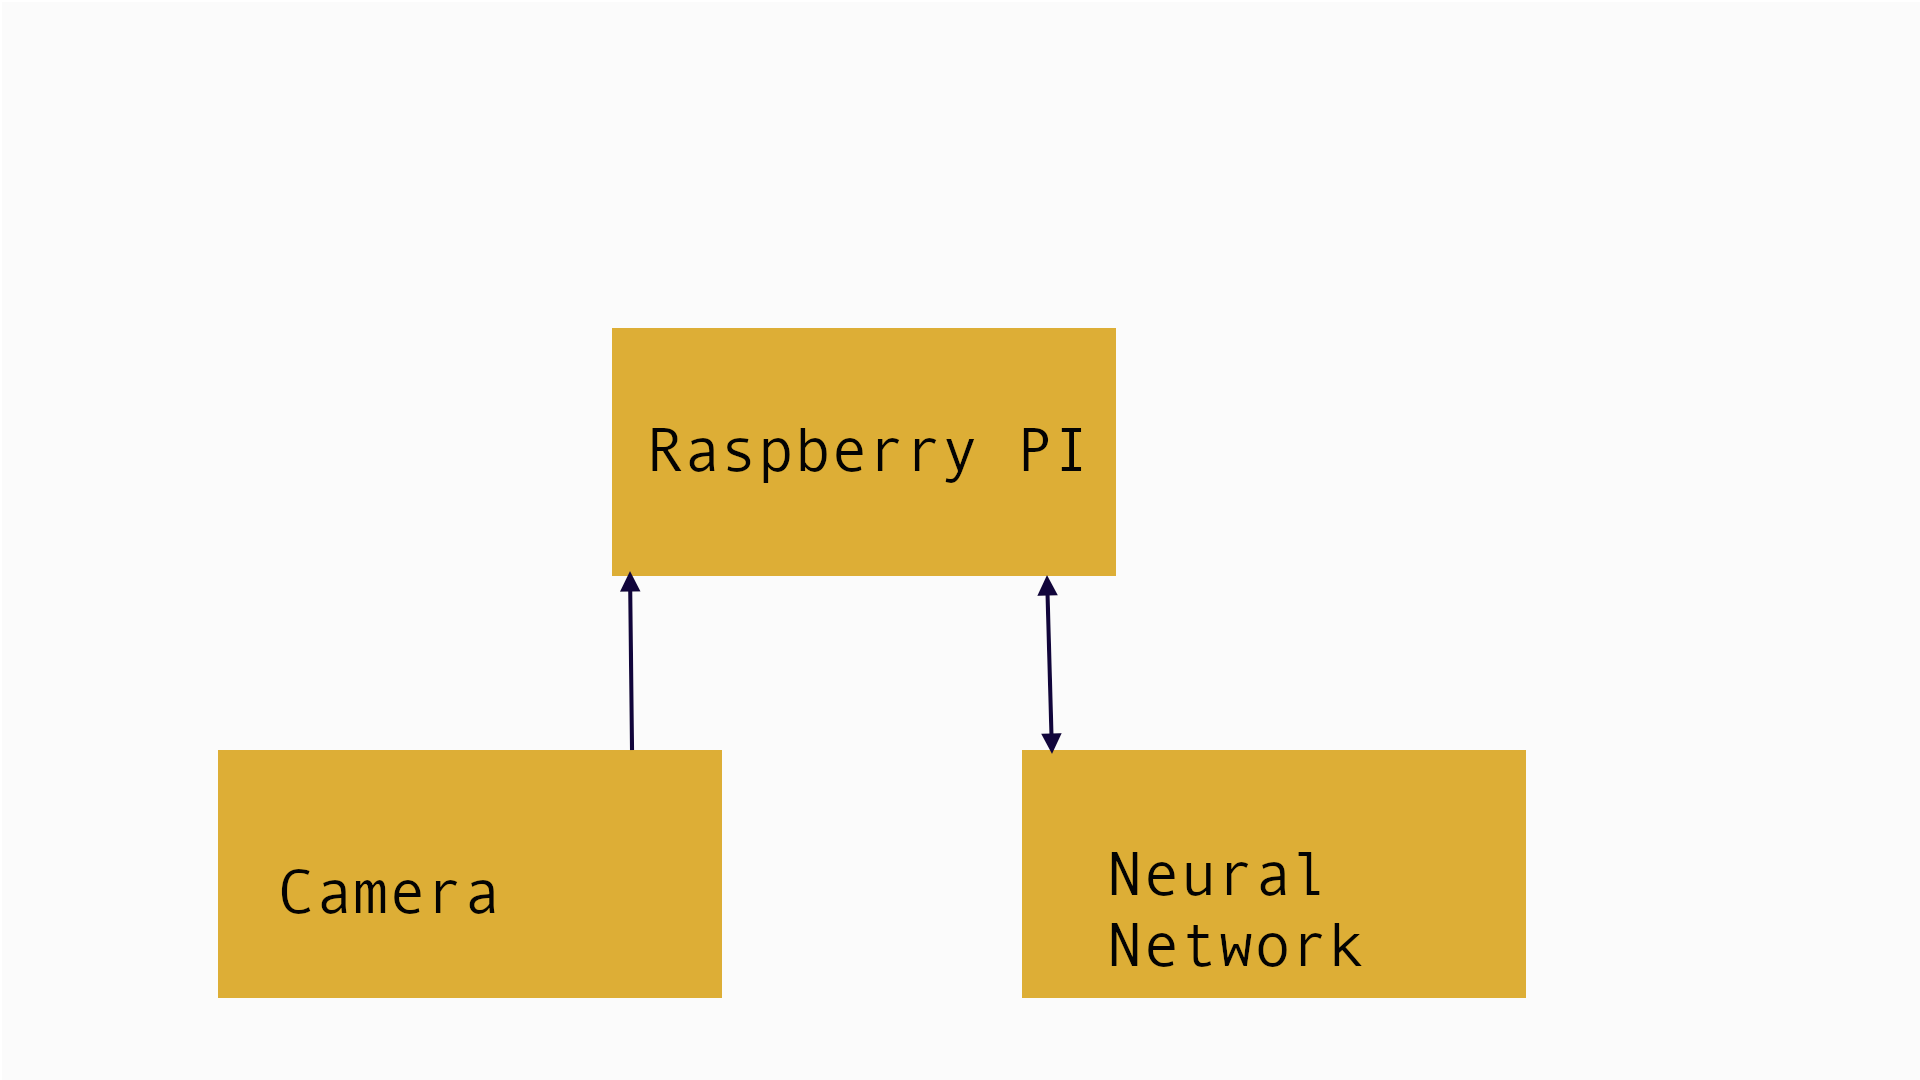
\includegraphics[scale=0.7]{block}
\caption{Different components of attention tracker}
\end{figure}

\subsection{Raspberry Pi}
The Raspberry Pi is a small single-board computer. It is developed by Raspberry Pi Foundation to promote teaching of basic computer science in schools. It has  1.2 GHz 64-bit quad core processor, on-board 802.11n Wi-Fi, Bluetooth and USB boot capabilities. 
\subsection{Camera}
The Raspberry Pi Camera Module v2 is a high quality 8 megapixel Sony IMX219 imagesensor custom designed add-on board for Raspberry Pi, featuring a fixed focus lens.
\subsection{Neural Network}
Neural network includes Image preprocessing block, feature extraction block and an implementation of deep learning network. Image processing works by convering the given image to integral image.
\subsubsection{Integral Image}
Integral image is the concept introduced by Viola Jones et al. It makes image processing faster. It is done by subjecting all the pixels of image to the following set of transformations.
\begin{align*}
    IntegralImage(x,y) &=Image(x,y)+IntegralImage(x-1,y)+IntegralImage(x,y-1)\\
    IntegralImage(x,-1) &=0\\
    IntegralImage(-1,0) &=0\\
\end{align*}
The resulting $IntegralImage$ is faster to perform image detection functions like the Haar Function. The Haar function selects rectangular regions in an image, and finds their difference from other
rectangular region.jj
